\section{Transport of concentrate}\label{se:transport_of_concentrate}

<<<<<<< HEAD
A model for transport of concentrate in sewer pipes is derrived in the following.

\begin{figure}[H]
\centering
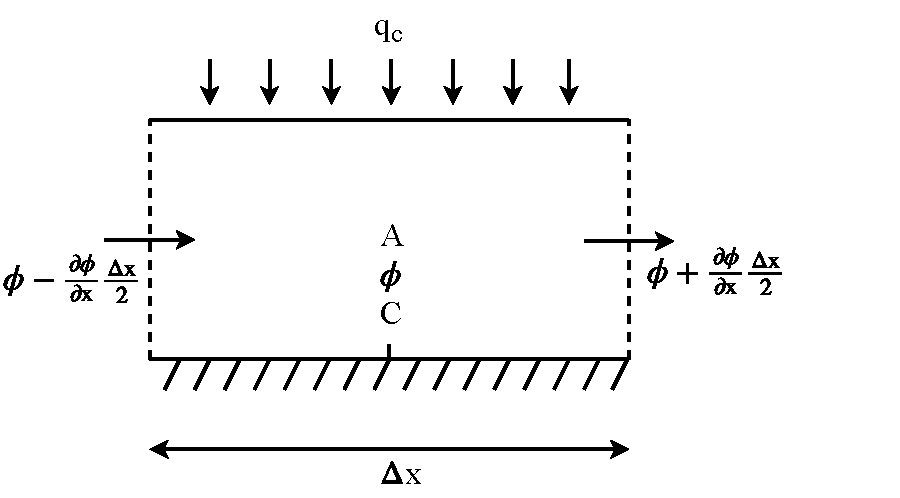
\includegraphics[width=.6\textwidth]{report/modeling/pictures/poopvolume.png}
\caption{Illustration of a control volume containing concentrate.}
\label{fig:poopvolume}
\end{figure} 
=======
 A derivation of a one dimensional model for transport of concentration, in channel flow, is given. 
 As in section \ref{se:hydraulics_of_sewer_line} certain assumptions is made when deriving the model.

 \begin{table}[H]
\begin{enumerate}
	\item The flow of concentrate is assumed to be steady and uniform in the cross section.
	\item The anoxic, anaerobic or aerobic processes occurring in the sewer line is neglected   
\end{enumerate}
\label{tab:concentrate_flow}
\end{table}
 In figure \ref{fig:concentrate_volume} the control volume is seen. 
>>>>>>> 32d1f724346e67c04c4c969a02fff176c83e23b5

 \begin{figure}[H]
\centering
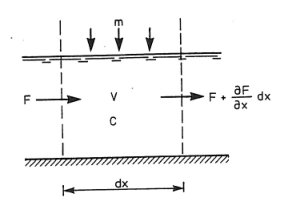
\includegraphics[width=.6\textwidth]{report/modeling/pictures/concentrate_volume.png}
\caption{Illustration of a control volume with concentrate.}
\label{fig:concentrate_volume}
\end{figure} 

From the control volume an equation for conservation of continuity can be derived as in section \ref{se:hydraulics_of_sewer_line}. The change of stored concentrate in the control volume is given as:

\begin{equation}
 \left(V \cdot C + \frac{\partial (V\cdot C)}{\partial t} \Delta t \right) - V\cdot C = \frac{\partial (V\cdot C)}{\partial t}\Delta t
\label{eq:poop_storing}
\end{equation}

Where V is the volume [$m^3$] and C is the concentrate [$\frac{g}{m^3}$]. 

The flux of concentrate in and out of the control volume at a given time $\Delta t$ is given as:


 \begin{equation}
  	\left( F_{in} - F_{out} + F_{lateral} \right) \Delta t   =	F \cdot \Delta t - \left(F + \frac{\partial F}{\partial x}\Delta x \right) \Delta t + m \cdot \Delta x \cdot \Delta t = - \frac{\partial F}{\partial x}\cdot \Delta x \cdot \Delta t +m \cdot \Delta x \cdot \Delta t  
  \label{eq:poop_flux_in_out}
  \end{equation} 



\fxnote{F er normalt en kraft, bare lige være sikker paa den ikke er taget}Where F is the flux [$\frac{g}{sec}$] and m is lateral flux input to the control volume [$\frac{g}{sec\cdot m}$].

The continuity equation can now be stated as the change in stored concentration equal to the sum of flux in- and outflow from the control volume as given by equation \ref{eq:poop_storing} and \ref{eq:poop_flux_in_out}:

\begin{equation}
	\frac{\partial (V\cdot C)}{\partial t}\Delta t = - \frac{\partial F}{\partial x}\cdot \Delta x \cdot \Delta t +m \cdot \Delta x \cdot \Delta t
\end{equation}

When replacing V with $\text{A}\cdot \Delta \text{x}$ and dividing with $\Delta x \cdot  \Delta t$ then the basic continuity equation of conservation is obtained:

\begin{equation}
	\frac{\partial (A\cdot C)}{\partial t} = - \frac{\partial F}{\partial x} + m 
\label{eq:concentrate_continuity_equation}
\end{equation}

Depending on the desired approximation the flux and lateral inflow terms can be expanded. The expanded lateral term describes a dead zone at the bottom the channel, which can be useful to model if dealing with rugged channel bed. Due to the prismatic assumption in \ref{se:hydraulics_of_sewer_line} of the sewer channel the dead zone in the channel is not investigated further. The flux terms describing convective flow and dispersion can be seen in table \ref{tab:flux_terms}.  

\begin{table}[H]
\centering
	\begin{tabular}{|l|l|l|} \hline
	Approximation 	& Convective flow &	Convective + (dispersion)  \\ \hline
	Flux term   	& $F = Q \cdot C$ & $ F = Q \cdot C + \left(- \epsilon \cdot A \frac{\partial C}{\partial x} \right)$  \\ \hline
  	\end{tabular} 
\caption{Table of convective flux term without and with dispersion where Q if flow, C is concentrate, A is area and $\epsilon$ is a dispersion coefficient [$\frac{m^2}{sec}$] .}
\label{tab:flux_terms} 
\end{table}

The dispersion term shown in the above table, also known as Fickian diffusion, gives an expression for how the molecules of the concentrate spreads. On a molecular level the the concentrate will to some degree disperse upstream and downstream as shown in figure \ref{fig:diffusion_example}. 

\begin{figure}[H]
\centering
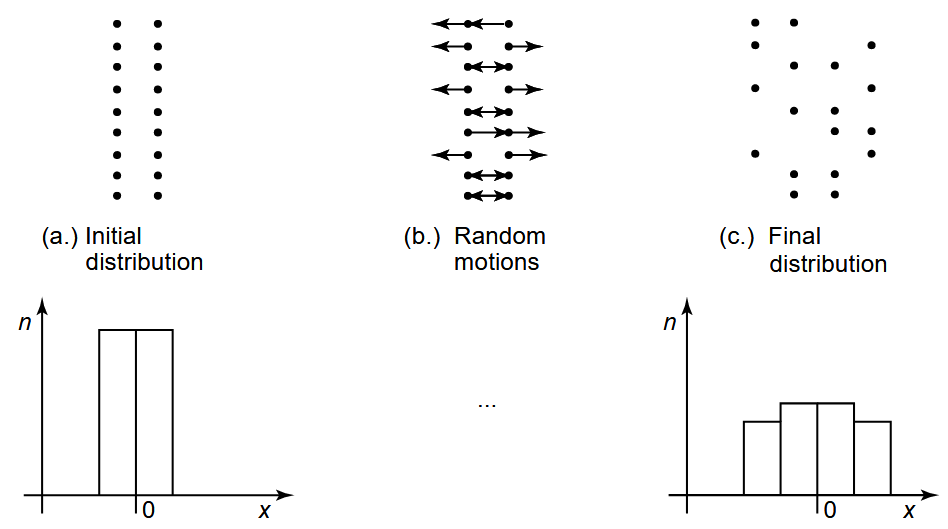
\includegraphics[width=.75\textwidth]{report/modeling/pictures/diffusion_example.png}
\caption{Illustration of distribution of convective flow without dispersion (a) and with (c), where dots illustrate molecules of the concentrate within a control volume \cite{karlruhe_con_def_dif_equation}.}
\label{fig:diffusion_example}
\end{figure} 

For various concentrates the dispersion coefficient $\epsilon$ which varies with temperature can be found in lookup tables \cite{karlruhe_con_def_dif_equation}.

Inserting the terms in table \ref{tab:flux_terms} into equation \ref{eq:concentrate_continuity_equation} then the following expressions of the continuity equation is obtained:

\begin{equation}
	\frac{\partial (A\cdot C)}{\partial t} + \frac{\partial (Q \cdot C)}{\partial x} = m 
\label{eq:concentrate_continuity_equation_convective}
\end{equation}

\begin{equation}
	\frac{\partial (A\cdot C)}{\partial t} + \frac{\partial (Q \cdot C)}{\partial x} - \epsilon \cdot \frac{\partial^2 (A \cdot C)}{\partial x^2} = m 
\label{eq:concentrate_continuity_equation_dispersion}
\end{equation}

